% Chapter 5
\chapter{Creating Your Own Panels}

In IzPack all of the actual work of installing an application is done in
panels.  The IzPack framework is primarily there to support the operation
of the panels and to manage the navigation through the installation
process.  This enables a user to decide which operations are carried out
during an installation and the order in which they are carried out, simply
by listing the appropriate panels in the desired order.\\

As far as extending the functionality of IzPack is concerned, the result
of this design is that new functionality can be integrated by adding new
panels to the framework and then listing them in the install spec.
Because the existing panels all have a visible GUI and because the term
panel hints at something visible, it is not obvious that a panel does not
have to contain any visible GUI to function in this framework.  There are
more details on this subject later on in this chapter.\\

\subsection{How to get started}

To get started with writing your own panels, it is best to place all the
IzPack code into a separate working directory, from where you can compile
it.  Then try to compile the code as is and get that to work.\\

The next step would be to have a look at another panel implementation, so you can
see how things are done.  Make sure you look at the less complicated panels,
as the panels with advanced features will only be confusing.  All the code
for building UI and such, only detracts from the essentials of what a panel
needs to do.  This means that you shouldn't start with
\texttt{UserInputPanel} or \texttt{ShortcutPanel}.  \texttt{HelloPanel} is
probably a much better choice at this stage.  The source code for panels
is located at:\\

\texttt{/src/lib/com/izforge/izpack/panels}.\\

You will find that all panels are derived from \texttt{IzPanel}; do the
same thing with your new panel.  Please note that the \texttt{IzPanel}
class itself is located in the \texttt{com.izforge.izpack.installer} package
but your panels need to belong to \texttt{com.izforge.izpack.panels}.
Perhaps you can just copy the code of a panel, remove all the functional
stuff and then start filling in your own code.  Start with something very
simple to begin with, just to see how it works.  The implementation is
really quite straight forward.\\

\subsection{Next Steps}

Once you have a successful compilation, you must place the compiled result
of your panel code at a special place, so that the installer compiler can
fetch it when building an installer that uses your panel.  Go to:\\

\texttt{/bin/panels}\\

You will see that there is a subdirectory for each panel.  Make a
subdirectory for your new panel with the exact same name as your panel and
place your compiled panel code there.\\

Once this is accomplished, you are ready to use your panel in an
installer.  Just list it in the spec file like any other panel, compile
and in theory it will show up when running the installer.  Once you made
it this far, you can dig deeper and get going with your specific needs.\\

Oh, and one other thing: If you think the your code might be useful for a larger
audience, please think about a contribution to IzPack.

\subsection{Access to the Variable Substitution System}

One thing many developers ask about is how to get access to the variable
substitution system.  This is not surprising, because customizing an
installation for a particular target environment is one of the most
important functions of an installer and the variable substitution system
plays a big part in this operation.\\

You can get access to the variable substitution system through the
protected variable \texttt{idata} in \texttt{IzPanel}.  This variable is
of the type \texttt{InstallData}, which is in turn subclassed from
\texttt{AutomatedInstallData}.  The Javadoc documentation will give you
more details on these classes.  Of particular interest in this context are
the methods \texttt{getVariable()}, \texttt{setVariable()} and
\texttt{getVariableValueMap()} in \texttt{AutomatedInstallData}.\\

\subsection{Controlling Flow}

Some of the interesting methods in
\texttt{com.izforge.izpack.InstallerFrame} that you might want to explore
are \texttt{lockPrevButton()} and \texttt{lockNextButton()}.  They allow
you to block the use of the button to move back to the previous panel
and the button that moves to the next panel respectively.  Being able to
control the availability of these buttons to the user is important if
one of your panels performs a task where the effects cannot be undone.  If
the user would navigate back to the previous panel your installation might
get into an unknown or even unstable state.  On the other hand, if the
operations in one panel vitally depend that a task in the previous panel
is completed, then you should block the use of the next button until that
task is completed.\\

\subsection{Reading XML}

If you need configuration files for your panel you would want to use XML
for that purpose.  To read XML files you should use NanoXML, as it is
guaranteed to be available at installation time.  In fact, all of the
IzPack infrastructure uses NanoXML to read XML files.  First you should
read the NanoXML documentation.  The documentation is included as PDF file
with the IzPack distribution, have a look in \texttt{/doc/nanoxml}.  In
addition to that, the Javadoc-generated class documentation is an
excellent resource to get help on NanoXML.  And then, there is always the
code of other panels to see practical examples.  Generally, it is a much
simpler matter to use NanoXML then to use the DOM included with the Java
distribution, so don't hesitate to explore NanoXML.

\subsection{Supporting Classes}

If your panel requires any supporting classes that are part of the panels
package, then you must place the *.class files into the same directory
with your panel .class file.\\

It is also possible to have supporting classes that are not part of the
panels package.  In fact, these classes don't even have to be in the
\texttt{com.izpack...} tree.  You simply have to ensure that the *.class
files are located in the proper directory structure inside
\texttt{/lib/installer.jar}.  If this is done, they will be available at
install time.  For your first experiments you can simply compile your
classes and add them to the *.jar file using the jar tool or a zip
utility.  However, ultimately it is much easier to use Ant and the IzPack
build script to accomplish this task.\\

\subsection{Panels that are not visible}

If you have a task that needs to be performed at a particular step in
the installation process, but that does not need any user interaction, you
can implement a panel that is not visible.  To implement this, you should
first familiarize yourself with the Javadoc documentation of
\texttt{com.izforge.izpack.InstallerFrame}.  In your panel code you get
access to the right instance of \texttt{InstallerFrame} through the
protected variable \texttt{parent} in \texttt{IzFrame}.\\

To begin with, do not configure any UI.  In other words, do not set a
layout and do not place any GUI elements on your panel.  In this context
the method \texttt{skipPanel()} is what gets the job done.  In your
\texttt{panelActivate()} method you simply perform your task and then call
\texttt{parent.skipPanel()}.  This gets the job done without the user
being aware that there was another panel in the flow.\\

\subsection{A word about building IzPack}

If you don't already use Jakarta Ant to support your development work, I
highly recommend you have a look at it.  It is a great help in organizing
practically all routine tasks connected with building and packaging your
application.  For example, building and getting IzPack ready for
distribution is not a straight forward process but with Ant this all comes
down to starting a single command.  In addition, IzPack provides its own
Ant task, which supports the integration of building a complete installer
into your regular build scripts.  You can find more details about this in
the chapter about advanced features.  To get a look at Ant you can visit
the following link: \url{http://ant.apache.org/index.html}.\\

You can find the Ant build script for IzPack itself at:\\

\texttt{/src/build.xml}\\

\section{The \texttt{IzPanel} Class}

\subsection{UML Diagram}

\begin{center}
\fbox{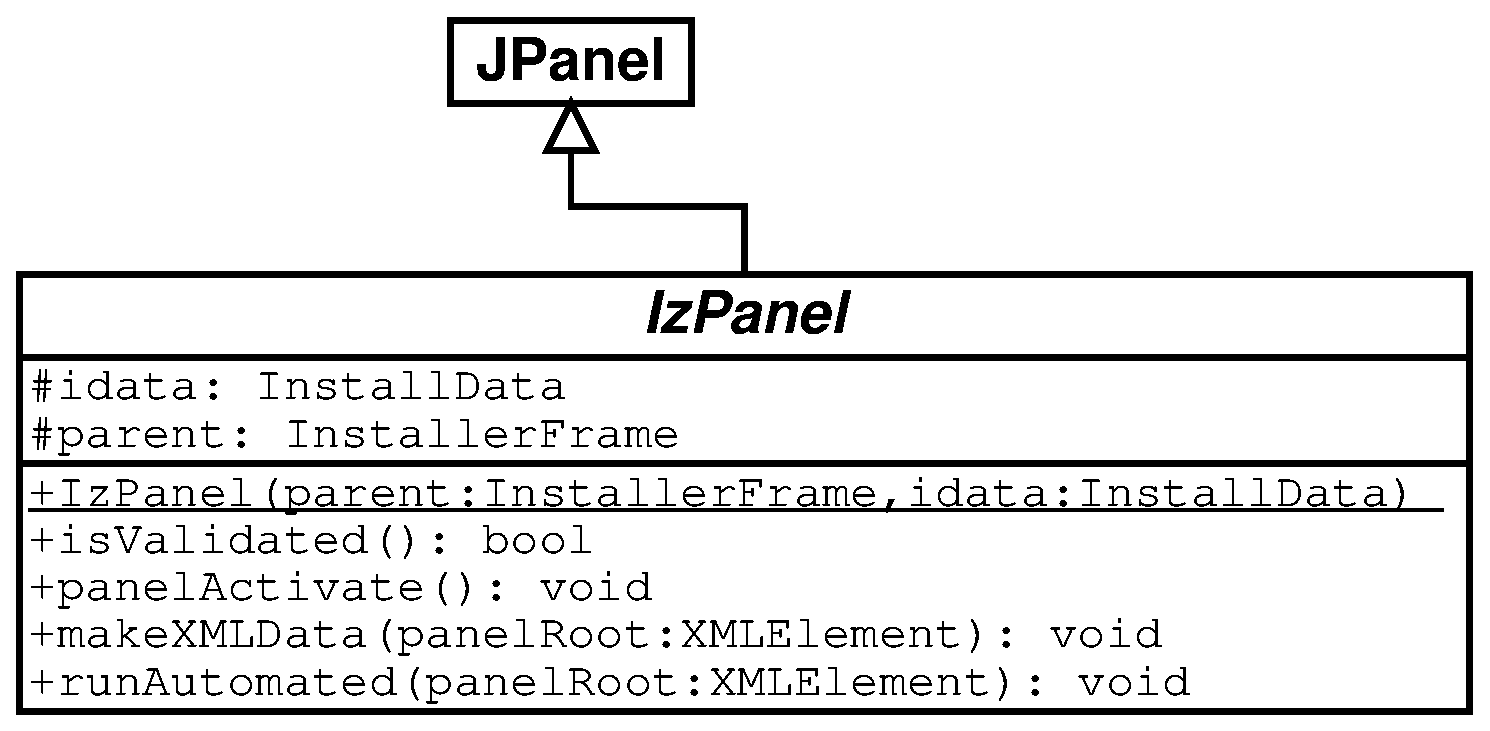
\includegraphics[scale=0.5]{img/ch5-izpanel}}
\end{center}\

\subsection{Description}

The two data members are : the install data (refer to the \texttt{InstallData}
Javadoc reference) and a reference to the parent installer frame.\\

The methods have the following functionality :\\
\begin{itemize}

  \item \textit{(constructor)} : called just after the language
  selection dialog. All the panels are constructed at this time and then
  the installer is shown. So be aware of the fact that the installer
  window is \textbf{not} yet visible when the panel is created. If you
  need to do some work when the window is created, it is in most cases
  better do it in \texttt{panelActivate}.\\

  \item \texttt{isValidated} returns \texttt{true} if the user is
  allowed to go a step further in the installation process. Returning
  \texttt{false} will lock it. For instance the LicencePanel returns
  \texttt{true} only if the user has agreed with the license agreement.
  The default is to return \texttt{true}.\\

  \item \texttt{panelActivate} is called when the panel becomes active.
  This is the best place for most initialization tasks. The default is
  to do nothing.\\

  \item \texttt{makeXMLData} is called to build the automated installer
  data. The default is to do nothing. \texttt{panelRoot} refers to the
  node in the XML tree where you can save your data. Each panel is given
  a node. You can organize it as you want with the markups you want
  starting from \texttt{panelRoot}. It's that simple.\\

  \item \texttt{runAutomated} is called by an automated-mode
  installation. Each panel is called and can do its job by picking the
  data collected during a previous installation as saved in
  \texttt{panelRoot} by \texttt{makeXMLData}.\\

  \item \texttt{setInitialFocus} with this method it is possible to set
  a hint which component should be get the focus at activation of the
  panel. It is only a hint. Not all components are supported. For more
  information see java.awt.Component.requestFocusInWindow or 
  java.awt.Component.requestFocus if the VM version is less than 1.4.\\
  
  \item \texttt{getInitialFocus} returns the component which should be get the
  focos at activation of the panel. If no component was set, null returns.\\

  \item \texttt{getSummaryBody} this method will be called from the 
  SummaryPanel to get the summary of this class which should be placed in the
  SummaryPanel. The returned text should not contain a caption of this item. 
  The caption will be requested from the method getCaption. If null returns, 
  no summary for this panel will be enerated. Default behaviour is to return 
  null.\\
  \item \texttt{getSummaryCaption} this method will be called from the 
  SummaryPanel to get the caption for this class which should be placed in the
  SummaryPanel. Default behaviour is to return the string given by langpack
  for the key ClassName.summaryCaption.\\
  

\end{itemize}\

Additionally, there are some helper methods to simplify grid bag layout handling
and creation of some common used components.

\section{The \texttt{Internationalization} of custom panels}
A common way to define language dependant messages for custom panels is to
add entries into the common langpacks which are stored in the directory
\begin{verbatim}
[IzPackRoot]/bin/langpacks/installer
\end{verbatim}
New with version 3.8 is the possibility to define a resource for custom
langpacks. Define e.g.
\begin{verbatim}
<resources>
    ...
    <res id="CustomLangpack.xml_deu" 
        src="myConfigSubPath/CustomLangpack_deu.xml"/>
    ...
</resources>
\end{verbatim}
in the install.xml file.The id should be written as shown, the file sub path
and name can be other than in the example. This file should be use the 
same DTD as the common langpack. For each language a separate file with
the ISO3 extension in the id should be used.

